\chapter{Olhó-passarinho}\label{chap:chap4}

Neste capitulo será abordado a ferramenta desenvolvida com a descrição da arquitetura sistema implementado, do processamento da informação espaço-temporal e da sua integração com a informação visual de modo a aplicar a tarefa de \textit{clustering}. Por fim será apresentado a visualização dos resultados ilustrativos e consequentemente a sua discussão. 

\section{Arquitetura do sistema}

A arquitetura do sistema desenvolvido é apresentado na figura~\ref{fig:archsys}. Este apresenta uma divisão entre os serviços externos e o modelo desenvolvido. Este modelo foi desenhado de modo a que existisse uma separação entre o tratamento de toda a parte de processamento dos dados e a visualização, existindo assim um \textit{back-end} com todos os ficheiros e módulos desenvolvidos e um \textit{front-end} que representa a aplicação web para visualização dos resultados. No \textit{back-end} existe também uma divisão entre dois módulos fundamentais, o módulo de processamento da informação visual, responsável por tratar a informação das imagens como descrito no Capítulo~\ref{chap:chap3}, de modo a que essa informação possa ser utilizada pelo módulo responsável pelo processo de \textit{Data Mining} já desenvolvido no TweeProfiles~\cite{Cunha2013}. 

Os serviços externos correspondem à base de dados Mongodb para a recolha dos tweets e os serviços Twitter e Instagram para a recolha das imagens através do URL. No caso do modelo desenvolvido, a parte de \textit{back-end} possuí os ficheiros JSON com os dados e as imagens necessárias, tanto para o módulo de processamento da informação visual como para a extração e processamento do dados espaço-temporais, explicados na próxima secção~\ref{sec:infoesptmp}. Os dados processados no módulo da informação visual e os dados espaço-temporal extraídos dos tweets são assim utilizados no processo de \textit{Data Mining}, onde é aplicada a tarefa de \textit{clustering} como explicado na secção~\ref{sec:finalclustering} apresentada mais adiante. De este processo resultam os \textit{clusters} calculados através de vários parâmetros, sendo estas informações armazenadas em ficheiros. Por fim, foi utilizada a \textit{microframework} Flask para desenvolvimento de aplicações web em Python, que permitiu o desenvolvimento da aplicação Olhó-passarinho para visualização dos resultados. 

\begin{figure}[h]
\centering
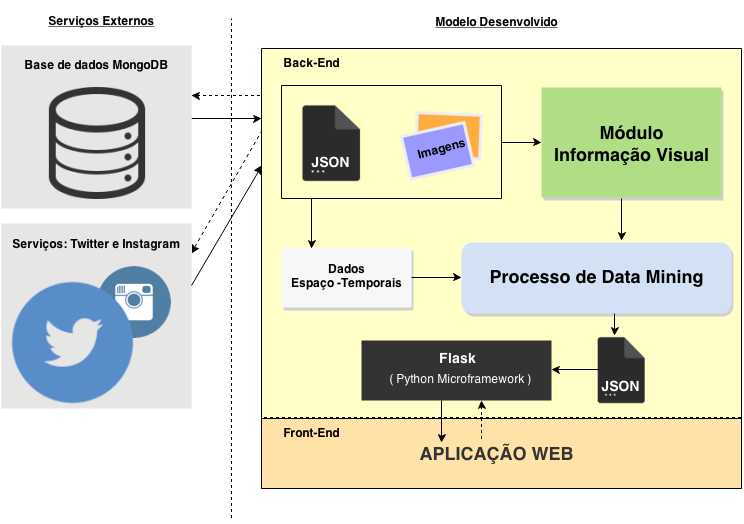
\includegraphics[width=1.0\linewidth]{./figures/arquitetura_sistema}
\caption{Arquitetura do sistema completo}
\label{fig:archsys}
\end{figure}


\section{Informação espaço-temporal} \label{sec:infoesptmp}

Uma das características principais tanto do TweeProfiles como do Olhó-paddarinho e é integração das dimensões espaço-temporais com o conteúdo. Tal como no foi efetuado no TweeProfiles, também aqui foi utilizado estas dimensões, tendo sido então recolhido a informação de tempo e espaço dos tweets para o cálculo das respetivas matrizes de distância entre tweets.

Em primeiro lugar foi recolhida a informação espacial. Neste caso os dados possuem a informação de latitude e longitude do ponto onde foi enviado o tweet. Para calcular a distância entre tweets utilizou-se a função distância Haversine abordada no capítulo~\ref{chap:estarte} na subsecção~\ref{subsubsec:space}. Neste caso foi calculada a distância em quilómetros, tendo sido considerado o valor do raio da Terra igual a 6371 Km.

Posteriormente foi então recolhida a informação temporal dos tweets. Esta informação apresenta-se no seguinte formato:

\vspace{2mm}
\centering\textbf{Tue Jun 18 17:02:09 +0000 2013}

Para o cálculo da distância entre data foi utilizada a distância a função distância euclidiana...


%\section{Clustering da informação visual, espacial e temporal} \label{sec:finalclustering}

%\section{Visualização}

%\section{Resultados ilustrativos}